% windsor's engineering notepad template
% uses emerald and lxfonts packages from ctan
%
% don't forget to change the date and other info in the header!!
%
% convert to bitmap with:
% convert -density 300x300 notes_template.pdf -resize 800x notes_template.png

\documentclass[12pt]{article}
\usepackage{CJK}
\usepackage[T1]{fontenc}
\usepackage{amsfonts}
\usepackage{emerald}
\usepackage{lxfonts}
\usepackage{amsmath}
\usepackage{graphicx}
\usepackage{eso-pic}
\usepackage{lastpage}
\usepackage[left=2.7cm,right=1.7cm,top=1.65cm,bottom=1.0cm]{geometry}





%��������������
\usepackage{mdframed}
\usepackage{enumerate}
\usepackage{multirow}

%����eps
\usepackage{graphicx}
\usepackage{epstopdf}
\usepackage{subfigure}

%������ַ
\usepackage{url}

%���볬����
\usepackage[colorlinks,linkcolor=blue]{hyperref}

%��ʽ����
\usepackage{amssymb,amsmath}


%�߿�

%������ɫ
\usepackage{color}





% configure page header
\usepackage{fancyhdr}
\setlength{\headheight}{15pt}
\pagestyle{fancy}\fancyhf{}
\renewcommand{\headrulewidth}{0pt}
\renewcommand{\footrulewidth}{0pt}
\lhead{\normalfont\ECFAugie \large{MATH 3E NOTES}}
\chead{\normalfont\ECFAugie \large{W. SCHMIDT}\hspace{1.4cm}}
\rhead{\normalfont\ECFAugie \large{\MakeUppercase{1/27/11}}\hspace{1.5cm}\thepage\hspace{0.1cm}/\hspace{0.1cm}\pageref{LastPage}\hspace{-1.5cm}}

% background image
\newcommand\BackgroundPic{
\put(0,0){
\parbox[b][\paperheight]{\paperwidth}{%
\vfill
\centering
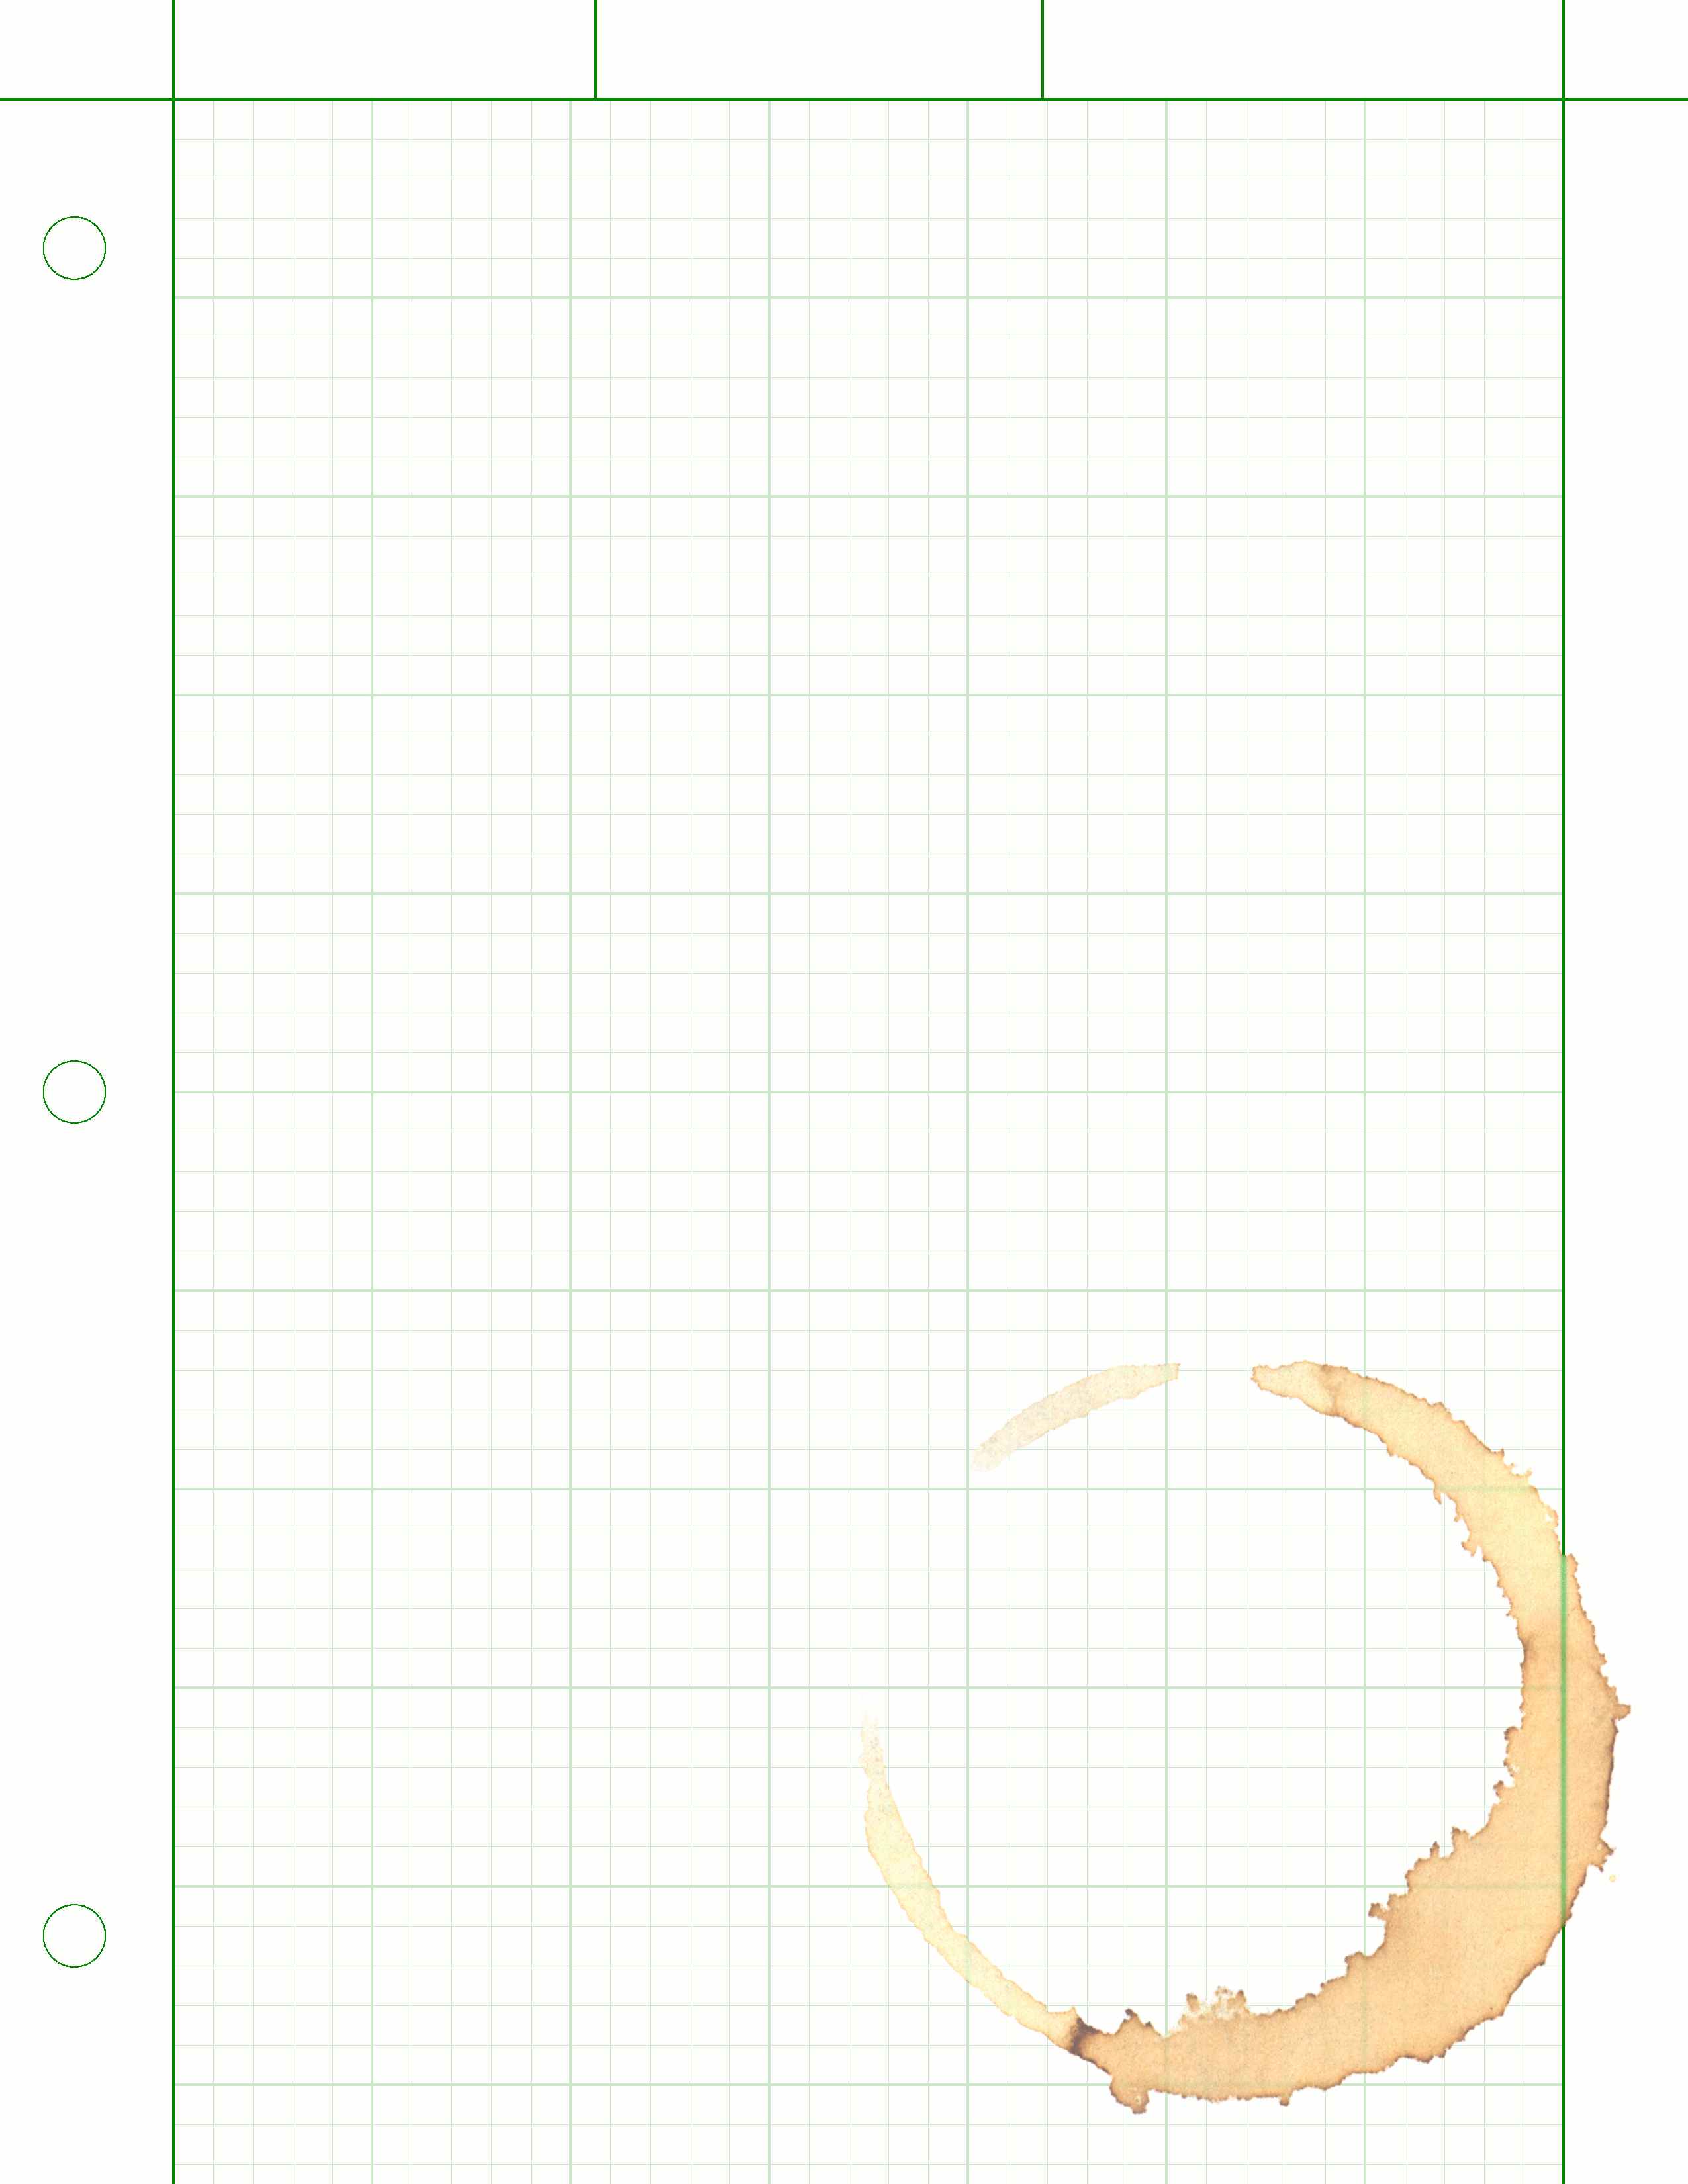
\includegraphics[width=\paperwidth,height=\paperheight,
keepaspectratio]{background.png}%
\vfill
}}}

% configure section titles
\usepackage{titlesec}
\titleformat{\section}{\Large}{\thesection}{1em}{}
\titleformat{\subsection}{\large\bfseries}{\thesubsection}{1em}{}

\begin{document}
\begin{CJK*}{GBK}{kai}
\AddToShipoutPicture{\BackgroundPic}
\normalfont\ECFAugie

% custom commands
\newcommand{\windef}[1]{\subsection*{\underline{DEF:} \normalsize{#1}}} % definition
\newcommand{\winex}[1]{\subsection*{\underline{EX:} \normalsize{#1}}} % example
\newcommand{\winsec}[1]{\section*{\underline{#1}}} % section
\newcommand{\winres}[1]{\begin{math}\Rightarrow\left\{\begin{matrix}#1\end{matrix}\right.\end{math}\hspace{0.2cm}} % result
\newcommand{\winsys}[1]{\begin{math}\left\{\begin{matrix}#1\end{matrix}\right.\end{math}} % system
\newcommand{\winero}[1]{\begin{math}\xrightarrow{#1}\end{math}} % row operation
\newcommand{\winmat}[1]{\begin{math}\begin{bmatrix}#1\end{bmatrix}\end{math}} % matrix
\newcommand{\winsub}[1]{\subsection*{$\star$\hspace{0.2cm} #1}} % dot
\newcommand{\step}[1]{\begin{math}\xrightarrow{\text{#1}}\end{math}} % step in a process
\newcommand{\winrtwo}{\begin{math}\text{R}^\text{2}\end{math}}
\newcommand{\winrthree}{\begin{math}\text{R}^\text{3}\end{math}}
\newcommand{\wineq}[1]{\begin{equation}\notag#1\end{equation}}

%���˼ӵ�
\newcommand{\winsubsub}[1]{\subsubsection*{$\quad \diamond$\hspace{0.2cm} #1}} % dot
%%%%%%%%%%%%%%%%%%%%%%
% start writing here %
%%%%%%%%%%%%%%%%%%%%%%



















\end{CJK*}
\end{document}
